\documentclass[11pt,a4paper]{article}
\usepackage{times}
\usepackage{latexsym}

\usepackage{url}

\usepackage{tikz-dependency}

  \usepackage{natbib}
  \bibliographystyle{plainnat}

\usepackage{CJKutf8}

%  \usepackage{natbib}
 % \bibliographystyle{plainnat}


\pagestyle{plain}

%\setlength\titlebox{5cm}
% You can expand the titlebox if you need extra space
% to show all the authors. Please do not make the titlebox
% smaller than 5cm (the original size); we will check this
% in the camera-ready version and ask you to change it back.

\newcommand\BibTeX{B{\sc ib}\TeX}
\newcommand\confname{EMNLP-IJCNLP 2019}
\newcommand\conforg{SIGDAT}

% Use the lineno option to display guide line numbers if required.

\usepackage{amsmath}
\usepackage{tikz-dependency}
\DeclareMathOperator*{\argmax}{arg\,max}
\DeclareMathOperator*{\argmin}{arg\,min}
\DeclareMathOperator{\E}{\mathop{\mathbb{E}}}

\usepackage{amssymb}% http://ctan.org/pkg/amssymb
\usepackage{pifont}% http://ctan.org/pkg/pifont
\newcommand{\cmark}{\ding{51}}%
\newcommand{\xmark}{\ding{55}}%

%\usepackage{pslatex}
%\usepackage{latexsym}
\usepackage[english]{babel}
\usepackage[utf8]{inputenc}
\usepackage{bm}
\usepackage{graphicx}
\usepackage{tikz}
\usepackage{xcolor}
\usepackage{url}
%\usepackage[colorinlistoftodos]{todonotes}
\usepackage{rotating}
\usepackage{multirow}





\usepackage[T1]{fontenc}

\usepackage{pslatex}
%\usepackage{latexsym}
\usepackage[english]{babel}
\usepackage[utf8]{inputenc}
\usepackage{amsmath}
\usepackage{bm}
\usepackage{graphicx}
\usepackage{tikz}
\usepackage{xcolor}
\usepackage{url}
%\usepackage[colorinlistoftodos]{todonotes}
\usepackage{rotating}
%\usepackage{natbib}
\usepackage{amssymb}

\usepackage{linguex}

\usepackage{amsthm}
 


\newcounter{theorem}
\newtheorem{proposition}[theorem]{Proposition}
\newtheorem{corollary}[theorem]{Corollary}
\newtheorem{question}[theorem]{Question}
\newtheorem{example}[theorem]{Example}
\newtheorem{defin}[theorem]{Definition}
\newtheorem{remark}[theorem]{Remark}
\newtheorem{lemma}[theorem]{Lemma}
\newtheorem{thm}[theorem]{Theorem}


\newcommand{\R}[0]{\mathbb{R}}
\newcommand{\Ff}[0]{\mathcal{F}}
\newcommand{\key}[1]{\textbf{#1}}


\newcommand{\soft}[1]{}
\newcommand{\nopreview}[1]{}
\newcommand\comment[1]{{\color{red}#1}}
\newcommand\mhahn[1]{{\color{red}(#1)}}
\newcommand{\rljf}[1]{{\color{blue}[rljf: #1]}}

\newcommand{\thetad}[0]{{\theta_d}}
\newcommand{\thetal}[0]{{\theta_{LM}}}
\newcommand{\thetap}[0]{{\theta_{P}}}
\newcommand{\japanese}[1]{\begin{CJK}{UTF8}{min}#1\end{CJK}}


\title{Dependency Length Minimization and Basic Word Order: A Corpus Study of Japanese}
\author{Michael Hahn \\ Stanford University \\ mhahn2@stanford.edu}
\date{\today}
\begin{document}
\maketitle
\begin{abstract}
The principle of Dependency Length Minimization holds that languages tend to exhibit word orders that reduce the length of syntactic dependencies.
Evidence for this hypothesis has been found in data from many languages, and it has been argued to accurately predict many phenomena across languages.
However, it appears to be at odds with the high typological frequency of SOV and VSO orders, as SVO orders would seem to provide shorter dependencies between verbs and their arguments.
We report a corpus-based study of Japanese that tests whether the typological frequency of SOV is compatible with Dependency Length Minimization.
In Study 1, we compare dependency lengths in real Japanese corpus data with a counterfactual SVO-like version of Japanese.
Results show that real Japanese with SOV order has shorter dependencies than the counterfactual SVO version.
In Study 2, we replicate this result using the Memory-Surprisal tradeoff, an information-theoretic measure of memory load in sentence processing that makes no assumptions about the format of syntactic representations. 
Taken together, the results show that the typological frequency of SOV is compatible with principles such as Dependency Length Minimization.
\end{abstract}


\section{Introduction}

There has been a suggestion that the typological distribution of word orders reflects a pressure towards efficiency of on-line syntactic processing.
Prominent among these proposals is the idea that syntactic structures are easier to process if syntactically related words are closer together in the surface string.
\cite{rijkhoff-word-1986} proposed a principle of \emph{Head Proximity}, arguing that head nouns tend to be close to the verbs governing them.
\cite{hawkins2014crosslinguistic} proposed a similar principle of \emph{Domain Minimization}, arguing that languages minimize the distances at which syntactic relations are established in a sentence.
The principle of \emph{Dependency Length Minimization} \citep{temperley2018minimizing} is a formalization of these ideas in terms of dependency grammar.

Dependency Length Minimization has been argued to explain Greenberg's harmonic correlations \citep{rijkhoff-word-1986, hawkins1994performance}, and certain kinds of exceptions, such as why pronominal objects pattern differently from nominal objects \citep{dryer1992greenbergian}. % JD: depending on where you plan to send this, you'll have to be mch more explicit about what this means
Hawkins \citep{hawkins2004efficiency, hawkins2007processing, hawkins2014crosslinguistic} has assembled further evidence that such principles predict specific word order facts in many languages. 
A prominent example is English Heavy NP Shift, which reduces the dependency length between verbs and objects by moving very long objects to the right of shorter dependents \citep{hawkins1994performance, wasow1997end}.
Japanese shows an analogous pattern, reducing dependency length by moving long objects earlier~\citep{yamashita2001long}.

Despite the success of Dependency Length Minimization, it appears to be at odds with the prevalence of SOV order \citep{ferrer-i-cancho-placement-2017}: In a sentence such as

\ex.
\begin{dependency}[theme = simple]
   \begin{deptext}[column sep=1em]
          She \& met \& friends  \\
   \end{deptext}
        %   \deproot{3}{ROOT}
   \depedge{2}{1}{subject}
   \depedge{2}{3}{object}
   %\depedge[arc angle=50]{7}{6}{ATT}
\end{dependency}

the overall dependency length is minimized by the English order, compared to SOV order as found in the Japanese
\ex.
\begin{dependency}[theme = simple]
   \begin{deptext}[column sep=1em]
          \japanese{彼女は} \& \japanese{友達に} \& \japanese{会った}  \\
          kanojo-wa \& tomodachi-ni \& atta \\ 
          she-\textsc{top} \& friends-\textsc{obj} \& met \\
   \end{deptext}
        %   \deproot{3}{ROOT}
   \depedge{3}{1}{subject}
   \depedge{3}{2}{object}
   %\depedge[arc angle=50]{7}{6}{ATT}
\end{dependency}

%JD This is rhetorically a bit unfortunate -- "appears" "entail" "should" "incorrectly" "predict" -- there are too many interactions between the semantics of these words to understand what a) DLT predicts, b) the facts are, c) the claim is that you're going to test. Split this up in a way that these three components become clear. Then it'll be easier to refer back to "the above claim"

One might conclude from these examples that Dependency Length Minimization predicts strong crosslinguistic prevalence of SVO order \citep{ferrer-i-cancho-placement-2017}.
This paper examines this claim, asking whether the prevalence of SOV orders indeed constitutes a challenge for Dependency Length Minimization.

First, does this conclusion remain true if we consider sentences more complex than the three-word one above? 
There may be sentences in which SOV order reduces length compared to SVO order:
This could happen in embedded clauses, in particular if subjects are similarly long or even longer than objects.
Depending on the frequency of different configurations in the language, such situations could outweigh cases in which SVO reduces length.
We therefore investigate which order reduces the \emph{average dependency length} over the \emph{distribution} of sentences as found in a corpus.
We will address this question by comparing the dependency length of actual Japanese orderings with counterfactual orderings exhibiting SVO order.
If actual Japanese sentences exhibit shorter average dependency length than these counterfactual orders, then this would provide evidence that -- given the syntactic structures actually occurring in Japanese -- the observed SOV order is best for Dependency Length Minimization.\footnote{Code and results for the studies described here are available at \url{https://github.com/m-hahn/japanese-sov}.}

Second, we ask which basic order improves processing efficiency
if we consider a more direct formalization of online memory limitations.
While Dependency Length Minimization is agreed to reflect working memory limitations in incremental processing \citep{hawkins1994performance, futrell2015largescale, temperley2018minimizing}, it does not directly formalize any psycholinguistically grounded quantity.
The actual, experimentally measured, processing effort induced by long dependencies is not a linear function of dependency length \citep{gibson1998linguistic}, and depends on intervening elements \citep{gibson1998linguistic, lewis-activation-based-2005} and the types of dependencies \citep{demberg-data-2008}.
As a more direct formalization of memory limitations, we will  investigate predictions made by 
the Memory-Surprisal Tradeoff \citep{hahn2019memory}, a purely information-theoretic bound on memory load in incremental processing that makes no assumption about the encoding of syntactic structure.
In Experiment 2, we test whether SOV order as found in Japanese results in more efficient memory-surprisal tradeoffs than a hypothetical SVO version.
If this is true, then this would provide evidence that a preference for SOV in Japanese is a prediction not only of Dependency Length Minimization, but of models positing memory limitations in online processing more generally.

\paragraph{Data}
We will base all our experiments on the Universal Dependencies \citep{nivre2019universal} treebanks.
This collection has three large Japanese treebanks (GSD, BCCWJ, KTC).\footnote{Two smaller corpora have no training partition, and were thus not used in this study.}
GSD and KTC reflect news text, these contain 7K and 6K sentences, respectively.
The much larger BCCJW (41K sentences) is based on the Balanced Corpus of Contemporary Written Japanese \citep{Maekawa2014}, reflecting a balanced selection of multiple genres.
Each corpus has a predefined split into three sets, a large training set, and two smaller held-out sets (\textit{dev} and \textit{test}).
We use the training set for our analyses, and leave other partitions for future experiments.


\paragraph{Basic Sentence Structure in Japanese}
This section will review basic facts about Japanese word order, serving as the background for the two corpus experiments.
Japanese is a strictly head-final language. The unmarked order is SOV; subjects, objects, and other modifiers all precede the verb.
NP dependents are marked with a case marker or postposition; for instance, \emph{ga} marks nominative, \emph{o} marks accusative, and \emph{wa} marks topics:

%\begin{huge}
%\textcolor{red}{TODO Japanese examples here}
%\end{huge}

\exg. [kodomo-tachi ga] [ano kooen de] [yakyuu o] suru \\
child-\textsc{pl} \textsc{nom} that park \textsc{loc} baseball \textsc{acc} do \\
`Children play baseball in that park' \citep[p. 118]{iwasaki2013japanese}

Tense, aspect, and mood markers follow the verb.
These elements are suffixes, though they are annotated as individual words in the Universal Dependencies \citep{nivre2019universal} treebanks, the source of our syntactically annotated corpus data:

\exg. [taroo ga] [ki o] taoshi-te-iru \\
Taro \textsc{nom} tree \textsc{acc} make.fall-\textsc{suff}-\textsc{asp:nopast} \\
`Taro is felling the tree' \citep[p. 138]{iwasaki2013japanese} \label{ex:taro-tree}

In terms of Universal Dependencies, this sentence would be rendered as follows:
\ex.
\begin{dependency}[theme = simple]
   \begin{deptext}[column sep=1em]
          \japanese{太郎} \& \japanese{が} \& \japanese{木} \& \japanese{を} \& \japanese{倒} \& \japanese{し} \& \japanese{て} \& \japanese{いる} \\
          taroo \& ga \& ki \& o \& tao \& shi \&te \& iru \\ 
   \end{deptext}
        %   \deproot{3}{ROOT}
   \depedge{1}{2}{case}
   \depedge{3}{4}{case}
   \depedge{5}{1}{nsubj}
   \depedge{5}{3}{obj}
   \depedge{5}{6}{aux}
   \depedge{5}{7}{mark}
   \depedge{5}{8}{aux}
   %\depedge[arc angle=50]{7}{6}{ATT}
\end{dependency}\label{ex:taro-tree-tree}

In accordance with the head-final order, all embedded clauses precede the verb; complementizers follow verbs, such as \textit{to} in this example:
\ex.
\begin{dependency}[theme = simple]
   \begin{deptext}[column sep=1em]
\japanese{太郎} \& \japanese{は} \& \japanese{花子} \& \japanese{が} \& \japanese{家出} \& \japanese{し} \& \japanese{た} \& \japanese{と} \& \japanese{嘆い} \& \japanese{た} \\
          taroo \& wa \& hanako \& ga \& iede \& shi \& ta \& to \& nagei \& ta \\ 
          Taro \& \textsc{top} \& Hanako \& \textsc{nom} \& leave.home \& do \& \textsc{past} \& \textsc{comp} \& grieve \& \textsc{past} \\
   \end{deptext}
   \depedge{9}{1}{nsubj}
   \depedge{1}{2}{case}
   \depedge{5}{3}{nsubj}
   \depedge{3}{4}{case}
   \depedge{5}{6}{aux}
   \depedge{5}{7}{aux}
   \depedge{5}{8}{mark}
   \depedge{9}{5}{xcomp}
   \depedge{9}{10}{aux}
   %\depedge[arc angle=50]{7}{6}{ATT}
\end{dependency}
`Taro grieved that Hanako had run away from home.' \citep[p. 224]{iwasaki2013japanese}\label{ex:hanako-ran}

% JD: Can you, based on these examples, already give the reader the intuition here explicitly for why SOV order might not be incompatible with DLM after all? 


\section{Experiment 1: Comparison of Dependency Length}


In Experiment 1, we will compare dependency lengths in real Japanese corpus data with a counterfactual SVO-like version of Japanese.

\subsection{Method}

%\paragraph{Japanese}
We based our experiments on the Universal Dependencies treebanks.
Following \cite{futrell2015largescale}, we converted these into a format closer to standard syntactic theory by promoting functional words
(conjunctions \texttt{cc}, 
postpositions \texttt{case},
copulas \texttt{cop},
complementizers \texttt{mark}) to heads \citep{osborne2019status}.
For instance, the example \ref{ex:taro-tree} above is converted as follows:
\ex.
\begin{dependency}[theme = simple]
   \begin{deptext}[column sep=1em]
          \japanese{太郎} \& \japanese{が} \& \japanese{木} \& \japanese{を} \& \japanese{倒} \& \japanese{し} \& \japanese{て} \& \japanese{いる} \\
          taroo \& ga \& ki \& o \& tao \& shi \&te \& iru \\ 
   \end{deptext}
        %   \deproot{3}{ROOT}
   \depedge{2}{1}{case}
   \depedge{4}{3}{case}
   \depedge{5}{2}{nsubj}
   \depedge{5}{4}{obj}
   \depedge{5}{6}{aux}
   \depedge{7}{5}{mark}
   \depedge{5}{8}{aux}
   %\depedge[arc angle=50]{7}{6}{ATT}
\end{dependency}


We restricted the experiment to the training partitions of each treebank, leaving the held-out partitions for future confirmatory research. 

Again following \cite{futrell2015largescale}, we measure the length of a dependency by the number of words intervening between head and dependent, plus one. 
The overall dependency length of a sentence is the sum of the lengths of all dependencies in that sentence.

We now describe how we constructed the counterfactual SVO-like version of Japanese.
%For each sentence in the treebanks, we compared its total dependency length to that of a version to which the following manipulation was applied: % why was this manipulation applied? what does it simulate? what do we gain by doing this?
In real (SOV) Japanese, subjects and subjects are ordered on the same side of the verb.
We obtained an SVO-like version by moving any subject, identified as the dependent of an \textit{nsubj} dependency, to the right of its head.
Heads sometimes have other dependencies to its right side, in particular verbs often have \textit{aux} dependents on the right.
We ordered the subject after these dependents.
This manipulation results in a version of Japanese that has OVS order.
Since dependency length is left-right invariant, it equally corresponds to an SVO version of Japanese, in which all phrases are strictly head-initial, and only subjects (\textit{nsubj}) and auxiliaries (\textit{aux}) precede their heads.
As subject NPs are mostly longer than auxiliaries (which always consist of one word), this method minimizes dependency length among all ways of placing the subject after the head, and thus biases \emph{against} our hypothesis that SOV worder is optimal for dependency length.
For instance, the example (\ref{ex:taro-tree}) above would become
\exg.  [ki o] taoshi-te-iru [taroo ga] \\
 tree \textsc{acc} make.fall-\textsc{suff}-\textsc{asp:nopast} Taro \textsc{nom}\\

\ex.
\begin{dependency}[theme = simple]
   \begin{deptext}[column sep=1em]
          \japanese{木} \& \japanese{を} \& \japanese{倒} \& \japanese{し} \& \japanese{て} \& \japanese{いる} \&  \japanese{太郎} \& \japanese{が}\\
          ki \& o \& tao \& shi \&te \& iru \& taroo \& ga\\ 
   \end{deptext}
        %   \deproot{3}{ROOT}
   \depedge{8}{7}{case}
   \depedge{3}{8}{nsubj}
   \depedge{2}{1}{case}
   \depedge{3}{2}{obj}
   \depedge{3}{4}{aux}
   \depedge{5}{3}{mark}
   \depedge{3}{6}{aux}
   %\depedge[arc angle=50]{7}{6}{ATT}
\end{dependency}\label{ex:taro-tree-tree-counter}



\ref{ex:hanako-ran} is converted to the counterfactual version
\ex.
\begin{dependency}[theme = simple]
   \begin{deptext}[column sep=1em]
 \japanese{家出} \& \japanese{し} \& \japanese{た} \& \japanese{花子} \& \japanese{が} \& \japanese{と} \& \japanese{嘆い} \& \japanese{た} \& \japanese{太郎} \& \japanese{は}\\
           iede \& shi \& ta \& hanako \& ga \& to \& nagei \& ta \& taroo \& wa\\ 
   \end{deptext}
   \depedge{7}{10}{nsubj}
   \depedge{10}{9}{case}
   \depedge{1}{5}{nsubj}
   \depedge{5}{4}{case}
   \depedge{1}{2}{aux}
   \depedge{1}{3}{aux}
   \depedge{6}{1}{mark}
   \depedge{7}{6}{xcomp}
   \depedge{7}{8}{aux}
   %\depedge[arc angle=50]{7}{6}{ATT}
\end{dependency}
`Taro grieved that Hanako had run away from home.' \citep[p. 224]{iwasaki2013japanese}\label{ex:hanako-ran-counter}




We first discuss under what circumstances we expect real or counterfactual Japanese lead to shorter dependency lengths. % JD: note

Comparison of \ref{ex:taro-tree-tree} and \ref{ex:taro-tree-tree-counter} suggests that, first, counterfactual orders will result in longer dependencies if there are many postverbal suffixes: The \textit{nsubj} dependency will be lengthened if the number of suffixes to the verb -- plus the length of the subject NP itself -- outweigh the number of words that intervene between subject and verb in real SOV orders, such as object NPs.
On the other hand, the length of the \textit{nsubj} dependency can be shortened if there are long constituents intervening in the SOV order, as in \ref{ex:hanako-ran}, where the subject \textit{taroo-wa} is separated from the verb by an embedded clause.
If subjects \emph{follow} other constituents depending on the verb, these dependencies will be shortened in counterfactual orders.

Second, comparison of \ref{ex:hanako-ran} and \ref{ex:hanako-ran-counter} shows that dependencies between complementizers and embedded verbs will be lengthened if the subject intervenes, as in \ref{ex:hanako-ran-counter}.

Clearly, which of the two orders results in shorter overall dependency lengths will depend on the relative distributions of different configurations in corpus data. % be more explicit -- what are the relevant configurations?

\subsection{Results}
In Table~\ref{tab:depl-resu}, we show the results for all three corpora.
We report average per-sentence dependency lengths for real (SOV) and counterfactual (SVO) orders.
We also report the $t$-value for the per-sentence difference between the two conditions.
In each of the corpora, the overall dependency length is lower on average in the original SOV orders than in counterfactual orders where subject and object are ordered on different sides of the verb.
The $t$ values indicate that all differences are highly reliable ($p < 0.0001$ in a two-sided $t$-test for the null that the mean difference is $0$).

We confirmed this using an exact binomial test, against the null that, conditional on there being a difference between the two conditions, dependency length is higher in  $\geq 50\%$ of cases.
This test confirmed our results, consistently rejecting the null ($p < 0.0001$) on each of the three datasets.


Note that the overall average difference is not large, corresponding to $\approx 1$ word.
This can in part be attributed to the fact that the averages is taken over all sentences in the corpus, and that many sentences show no difference in dependency length between real and counterfactual orders.

In Figure~\ref{fig:memsurp-jap}, we show the distribution of dependency length reduction of SOV order vs. counterfactual SVO order.
Again the difference between the two groups appears relatively small visually, but the analyses show that this difference is statistically reliable both in terms of the \emph{number of sentences} that show a dependency length reduction in the real order, and in terms of the \emph{average reduction} of dependency length.





\begin{table}
\begin{center}
\begin{tabular}{l|l|lllllll}
 Corpus                   &   Sents.                     & O,S same side   & O, S different sides  & $t$   \\ \hline\hline
All Corpora     &  54K     & 61.65 & 62.66 &   15.22   \\ \hline
GSD             &   7K       & 51.64 &  52.92  &  10.18  \\
BCCWJ           &   41K       &    63.04   & 63.97 &  11.39  \\
KTC             &   6K   &  64.01 & 65.27 &  7.45\\ \hline
\end{tabular}
\end{center}
\caption{Dependency Lengths for Japanese. For each corpus, we show the number of sentences, and average overall dependency length for the real orders (O, S on the same side of the verb), and the counterfactual orders (O, S on different sides of the verb).}\label{tab:depl-resu}
\end{table}



\begin{figure}
    \centering
    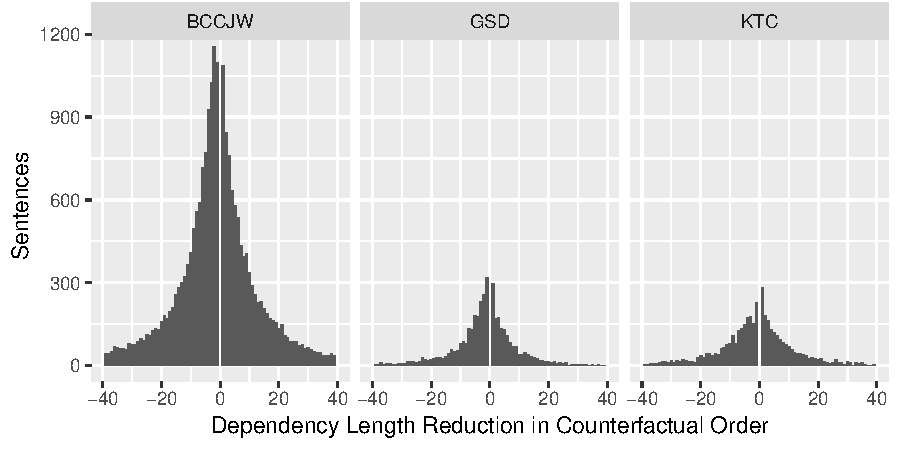
\includegraphics[width=0.9\textwidth]{figures/dependency_lentgh_differences_byCorpus.pdf}
\caption{Dependency Length Difference between real (SOV) and couterfactual (SVO) orders, conditioned on the difference being nonzero. For legibility, we clipped the $x$-axis at 5\% quantiles of the BCCJW corpus. Sentences to the left of $x=0$ have shorter dependency length in real orders, sentences to the right have shorter length in counterfactual orders. }\label{fig:memsurp-jap}
\end{figure}




\subsection{Discussion}
We found that SOV orders reduce average dependency length compared to counterfactual SOV orders, when applied to Japanese corpus data.
How does this overall difference relate to specific dependencies? 
As discussed above, we hypothesize that real orders reduce dependency length between verbs and elements that embed them -- i.e., matrix verbs (\emph{acl}), complementizers (\emph{mark}, \emph{case}), and copulas (\emph{cop}).
We therefore expect that the lengths of the \emph{acl}, \emph{mark}, \emph{case}, and \emph{cop} dependencies are \emph{reduced} in real orders.

Furthermore, as discussed above, we hypothesize that they \emph{increase} dependency lengths between verbs and those elements that tend to appear to the left of subjects, such as the various types of adverbial modifiers (such as \textit{advmod}, \textit{obl}), and left-dislocated elements (\textit{dislocated}).

We investigated this using the GSD corpus.
For each dependency type, we calculated how much dependency length is reduced on average by the real orders.
Results are shown in Table~\ref{fig:shortened} (for dependencies with overall length reduction) and Table~\ref{fig:shortened} (for dependencies with overall length increase).
In agreement with the predictions, we find reliable mean reductions for the \emph{acl}, \emph{mark}, \emph{case}, and \emph{cop} dependencies.
We also find strong reduction for the \emph{nsubj} dependencies.


Regarding increases, we find the strongest mean increases for relations representing elements occurring to the left of objects, similar to subjects (\emph{advmod}, \emph{dislocated}, \emph{obl}, \emph{advcl}, \emph{iobj}, \emph{csubj}, \emph{nmod}).
This again is in agreement with the prediction that dependency lengths should be inreased in SOV order for elements that tend to appear to the left of subjects in Japanese.

\begin{table}
\begin{center}
\begin{tabular}{l|llllllllll}
   Dependency  &Number &Reduction     &  Mean   &   SD &       $t$ \\ \hline
  case & 35257  &  99\% & -0.0402     &0.660  & -11.4   \\
 compound     &14383  &  100\%     & -0.000139   &0.0118 &  -1.41  \\ 
 mark  & 7616  &  0.99\% & -1.44       &3.50 &   -35.8   \\
  nsubj        & 5880  &  67\% & -1.34       &8.69  &  -11.8   \\
  acl          & 5225  &  100\%     & -0.509      &2.08  &  -17.7   \\
 cop   & 1843  &  100\%    &  -0.966      &2.70  &  -15.3   \\
 det          &  705  &  100\%    &  -0.0113     &0.301 &   -1.000 \\
 amod         &  694  &  100\%    &  -0.0144     &0.380 &   -1.000 \\
\end{tabular}
\end{center}
\caption{Dependencies that are shortened in real orders, compared to counterfactual orders. For each dependency type, we show how many occurrences there are (Number), how often the length is reduced, as opposed to increased (Reduction), the mean change in length (Mean), and the SD and $t$ statistics of the change. Greater absolute values of $t$ indicate more reliable changes in dependency length.}\label{fig:shortened}
\end{table}


\begin{table}
\begin{center}
\begin{tabular}{l|llllllllll}
   Dependency  &Number &Reduction     &  Mean   &   SD &       $t$ \\ \hline
  aux      &    18395  &  33\% &  0.0000544  &0.0128 &   0.577 \\
 nmod         &12651  &  2\%&  0.0150     &0.335  &   5.04  \\
 obl          & 7921  &  0\%     &  0.687      &2.51&     24.4   \\
  advcl        & 7445  &  33\% &  0.396      &3.24  &   10.5   \\
 obj          & 4364  &  0\%     &  0.0266     &0.361 &    4.86  \\
 iobj         & 4068  &  0\%    &  0.611      &2.15  &   18.1   \\
 nummod       & 3676  &  0\%     &  0.000544   &0.0330&    1.000 \\
 advmod       & 2300  &  1\%&  1.16       &3.50  &   15.9   \\
 csubj        &  444  &  0\%    &   0.113      &0.696 &    3.41  \\
 ccomp        &  336  &  0\%    &   0.00893    &0.164 &    1.000 \\
 dislocated   &  177  &  0\%    &   5.49       &4.53  &   16.1   \\
\end{tabular}
\end{center}
\caption{Dependencies that are lengthened in real orders, compared to counterfactual orders. See Figure~\ref{fig:shortened} for explanation of column names.}\label{fig:lengthened}
\end{table}



\section{Experiment 2: Memory-Surprisal Tradeoff}

In Experiment 1, we found that Dependency Length Minimization, applied to syntactic structures of Japanese as found in dependency treebanks, favors the observed SOV order over counterfactual SVO-like orders.
However, dependency length presupposes a specific representation format of syntactic structures, and may not be robust to different versions of dependency grammar.
The results from Experiment 1 might therefore be dependent on the analysis choices expressed in Universal Dependencies annotation.


Furthermore, dependency length does not directly reflect a measure of memory load, as actual processing effort induced by long dependencies is neither linear in length, nor independent of factors such as the intervening words and the type of dependency \citep{gibson1998linguistic,lewis-activation-based-2005,demberg-data-2008}.

To address these concerns, we now turn to a measure of processing under memory limitations that does not depend on the syntactic analysis, namely the Memory-Surprisal Tradeoff \citep{hahn2019memory}.
This is based on the observation that listeners who maintain imperfect memory of the input will incur higher surprisal than listeners who maintain more detailed memory representations.
This results in a tradeoff between memory and surprisal:
For each budget of memory, quantified by the number of bits that a listener uses to encode information about the past, there is a minimal amount of surprisal that this listener will incur on average.
Languages enable more efficient processing under memory limitations if this tradeoff is more favorable -- that is, if a listener with any fixed memory budget can achieve low surprisal.

This tradeoff can be estimated using information-theoretic bounds that are independent of assumptions about how syntactic structure is encoded \citep{hahn2019memory}.
For any $t = 1, 2, \dots$, let $I_t$ be the Conditional Mutual Information of two words $X_0, X_t$ conditioned on the intervening words:
\begin{equation}
        \operatorname{I}_t := \operatorname{I}[X_t, X_0 | X_1, \dots, X_{t-1}] = \operatorname{H}[X_t|X_1, \dots, X_{t-1}] - \operatorname{H}[X_t|X_0, \dots, X_{t-1}] 
\end{equation}
This quantity  measures how much predictive information is provided by the next word $X_t$ by the word $t$ steps in the past.
It is a statistical property of the language, and can be estimated from text data.

\citet{hahn2019memory} show that a listener who invests at most $\sum_{t=1}^T t I_t$ bits of memory will incur average surprisal at least $H[X_t| X_{<t}] + \sum_{t=T+1}^\infty I_t$.
By tracing out all values $T >0$, one can obtain a bound on the tradeoff curve for any possible listener.

\paragraph{Setup}
We estimated the Conditional Mutual Information $I_t$ (for $t=1,2,\dots,20$) using standard estimation methods for language modeling based on neural networks~\citep{hochreiter-long-1997}, as described in \citet{hahn2019memory}.
This estimation method is based purely on surface strings, without any structural assumptions.

We then used the theoretical result described above to compute memory-surprisal tradeoff curves of real and counterfactual orderings.

We could only use the GSD treebank here (7K sentences), as the others come only with POS and dependency annotation, with the original words removed due to copyright restrictions.

We estimate a single model for both versions (real and counterfactual), trained on a version of Japanese where each sentence is either left unachanged or manipulated, at random.
We then evaluate the resulting model separately on held-out data according to the two versions (original or manipulated).
By controlling for differences between different random initializations, this method increases statistical precision in estimating differences between the two versions of Japanese.
We estimated 20 such models to control for differences between random initializations.

We also conducted an analogous study for English.
It might be the case that SOV orders improve memory-surprisal tradeoffs across languages.
Repeating the study for English controls for this:
If word orders provide efficient memory-surprisal tradoffs, then SVO order will provide more favorable memory-surprisal tradeoffs for English data than counterfactual SOV orders.
We use the Penn Treebank~\citep{marcus-building-1993}.
For counterfactual orders, we order subject NPs (\texttt{NP-SBJ}) after VPs (\texttt{VP}), producing VOS order.
Again, since the memory-surprisal tradeoff curves are left-right invariant, this is equivalent to SOV order.


\paragraph{Results}

Results are shown for Japanese in Figure~\ref{fig:memsurp-jap}, and for English in Figure~\ref{fig:memsurp-ptb}.
In both languages, the real orders show better memory-surprisal tradeoffs than the counterfactual ones, in every one of the 20 runs of the LSTM language model.

In terms of the size of the effect, the difference between the two versions is considerably larger in Japanese than in English.
Nonetheless, the English result confirms that language-specific properties influence which basic word order provides better memory-surprisal tradeoffs.


\begin{figure}
    \centering
    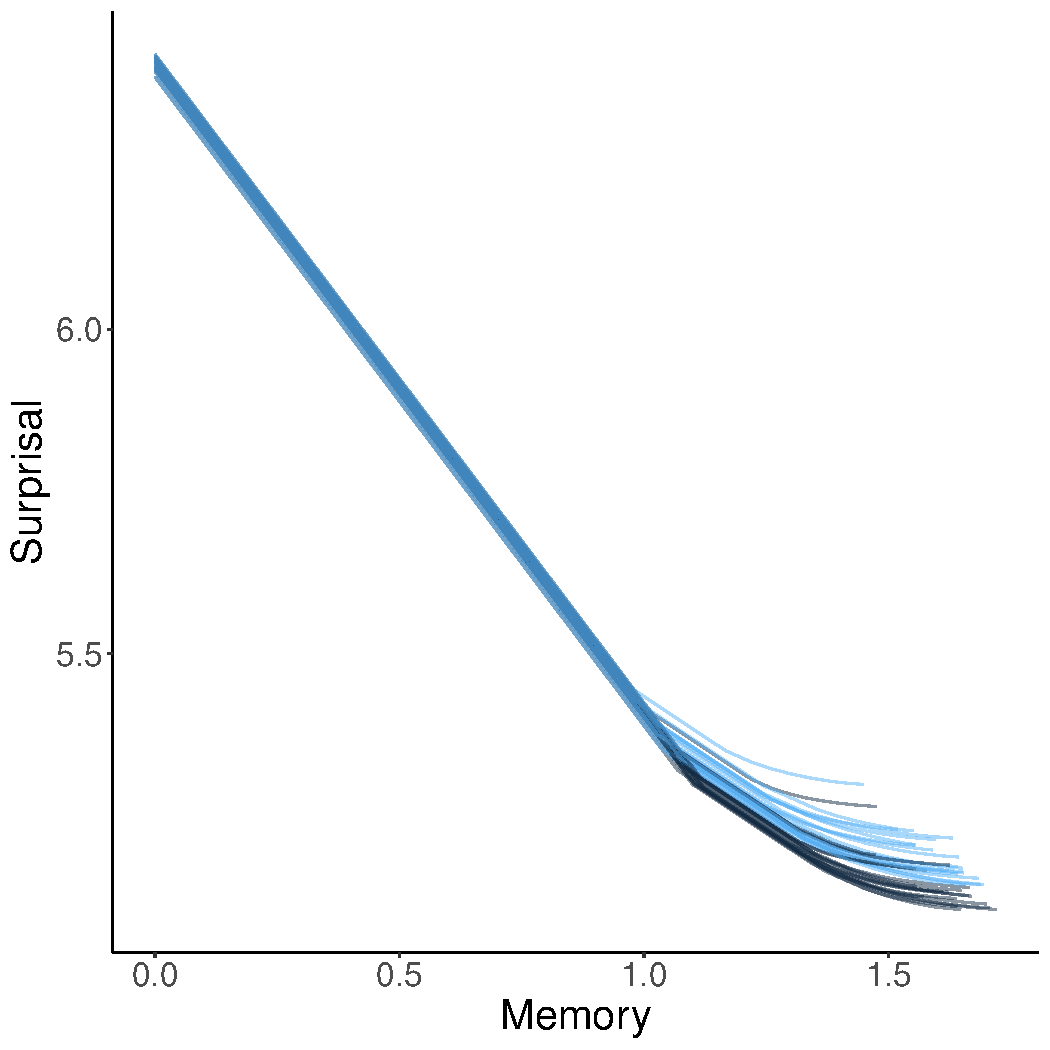
\includegraphics[width=0.6\textwidth]{figures/japanese-memsurp.pdf}
\caption{Memory-surprisal tradeoff for Japanese, for the 20 runs of the language model. Dark blue: real orders (object and subject on the same side of the verb). Light blue: counterfactual orders (object and subject on different sides of the verb).}\label{fig:memsurp-jap}
\end{figure}


\begin{figure}
    \centering
    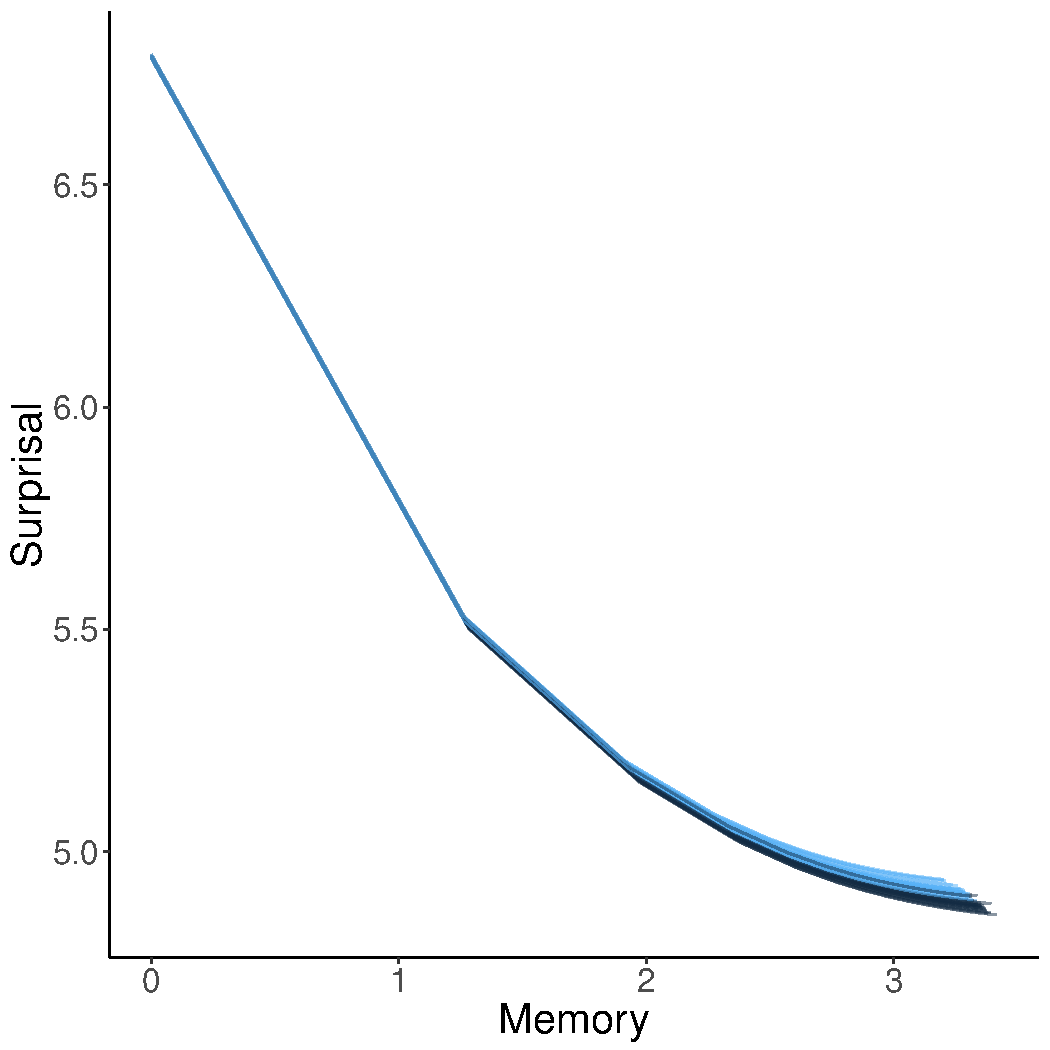
\includegraphics[width=0.6\textwidth]{figures/ptb-memsurp.pdf}
\caption{Memory-surprisal tradeoff for English (Penn Treebank), for the 20 runs of the language model. Dark blue: real orders (object and subject on the different sides of the verb). Light blue: counterfactual orders (object and subject on the same side of the verb).}\label{fig:memsurp-ptb}
\end{figure}


\section{Discussion}


We found evidence that SOV order as found in Japanese reduce memory load in processing, using two quantitative models of memory load: Dependency length and the Memory-Surprisal tradeoff.
These results suggest that the observed prevalence of SOV order is not at odds with Dependency Length Minimization and similar locality principles.
Instead, these principles interact with the language-specific distribution of syntactic structures to make language-specific predictions about which word order should be preferred on processing grounds.


A limitation of this study is that our counterfactual SVO version of Japanese might have properties that distinguish it from actually occurring SVO languages,
and might therefore be unrealistic as a comparison baseline. 
For instance, in SVO languages, certain adverbs (e.g., high-scoping ones) precede the verb together with the subject, and others (e.g., manner adverbs) follow it, together with the object.
For instance, in English, manner adverbs (e.g., \emph{quickly}) may follow or precede the verb. Speaker-oriented adverbs (e.g., \emph{fortunately}) tend to occur before the verb.
In this study, we created a counterfactual SVO version of Japanese in which all adverbs uniformly follow the verb.
The available UD annotation does not make it possible to easily identify adverbs that might typically precede the verb in an SVO language.



The observed dependency length reduction in real Japanese orders seems small, being approximately 1 word per sentence.
The question arises whether such a difference is sufficient as a pressure constraining language change.
Finding ways to estimate what effect sizes might be needed to shape language change is an important question for future work.
One path to study this might using artificial language experiments, which can be used to understand how efficiency pressures influence language change  \citep{fedzechkina2012language}.


%A common limitation of studies based on treebank data is that the data comes from written sources, whereas pressures coming from cognitive constraints arguably shape spoken language in language change.
%Annotating spoken data, or behavioral experiments could alleviate this concern in future work. % JD why is this a limitation, given that you're talking about a synchronic snapshot of the language? or say a little more about why this is or isn't a worrisome limitation



\section{Conclusion}
We examined the question whether the typological prevalence of SOV order constitutes a problem for the idea that crosslinguistic word order distributions reflect optimization for processing under memory constraints.
We found that this is not the case: Word orders found in English and Japanese are optimal for the respective languages, as they reduce average dependency length and memory load compared to counterfactual orderings.
The results highlight that predictions of efficiency principles for language structure have to be evaluated against specific data from languages, and that they can have language-specific consequences even in domains that are crosslinguistically relevant, such as basic word order.
Our methodology is applicable crosslinguistically, and future work should apply it both to other languages, and to other phenomena where efficiency principles might make language-specific predictions.


\bibliography{literature}
%\bibliographystyle{acl_natbib}


\end{document}





\section{Experiment 1: Optimization}

recycle QP experiment

here present the optimized grammars side-by-side



\section{Experiment 3: What Factors are Responsible?}

- all NPs are strictly head-final, and have final case marker

- almost all verbs are `embedded'

-- either with auxiliary

-- or with something else



\begin{center}
\begin{tabular}{lllllllll}
                    &                        & O,S same side   & O, S different sides    \\ \hline\hline
Ordinary UD         & Plain                  & 53.34 & 53.09\\
                    & Reordering Siblings    & 45.99 & 48.02 \\ \hline
Removing FuncWords  & Plain                  & 23.85 & 23.53 \\
                    & Reordering Siblings    & 19.68 & 20.71 \\ \hline
FuncHead UD         & Plain                  & 51.81 & 53.24 \\ % (excluding aux)
                    & Reordering Siblings    &  TODO     &  \\ \hline
FuncHead UD+Aux         & Plain                  & 67.86 & 69.25 \\ % (including aux) TODO this faces the problem that stacked AUX might be analyzed in the wrong order
                    & Reordering Siblings    &  TODO     & \\  \hline 
\end{tabular}
\end{center}


\begin{table}
\begin{tabular}{l|rlll}
Name & Words & Available\\ \hline
GSD     & 184K & full\\
PUD     & 26K & full\\
Modern & 14K & full\\
BCCWJ & 1,237K & POS+deps\\
KTC & 189K & POS+deps \\
\end{tabular}
\end{table}




2.4 total: 54K sentences

Functional Heads:

cc: \begin{CJK}{UTF8}{min}と, や\end{CJK}

case: doesn't apply to verbs\footnote{https://universaldependencies.org/ja/dep/case.html}

cop: \begin{CJK}{UTF8}{min}だ\end{CJK} 

mark: \begin{CJK}{UTF8}{min}と, か\end{CJK} 

Method for bringing S to the other side: sorting it after the other dependents, as these are short (auxiliaries etc).

\paragraph{English}